%============================ MAIN DOCU =================================
% define document class
\PassOptionsToPackage{table}{xcolor}
\documentclass[
   10.5pt,
   invert-title=true,
   titlepage=false,
   titleimage-ratio=13,
   class=article
]{bfhpub}				% KOMA-script report
%---------------------------------------------------------------------------
% Documents paths
%---------------------------------------------------------------------------
\makeatletter
\def\input@path{{content/}}
%or: \def\input@path{{/path/to/folder/}{/path/to/other/folder/}}
\makeatother
%-----------------  Set default font family  -------------------------------
\renewcommand{\familydefault}{\sfdefault}
%-----------------  Base packages     --------------------------------------
% Include Packages
\usepackage[babel, german=quotes]{csquotes}
%---------------------------------------------------------------------------
\usepackage{blindtext}  %% For placeholder text only
%---------------------------------------------------------------------------
\usepackage{geometry}
\geometry{
   a4paper, % Papierformat
   top=3cm, bottom=4cm, % Rand oben/unten
   outer=2.5cm, inner=3cm % aussen/inne
}
%---------------------------------------------------------------------------
%\usepackage[
%  backend=biber,
%  style=alphabetic,
%  sorting=ynt
%]{biblatex}
%\addbibresource{sample.bib} %% Name of bibliography file
%---------------------------------------------------------------------------
\usepackage{multicol}
%---------------------------------------------------------------------------
% Hyperref Package (Create links in a pdf)
%---------------------------------------------------------------------------
\usepackage[
   hidelinks
  ,colorlinks
  ,linkcolor=.
  ,filecolor=.BFH-MediumGreen
  ,urlcolor=BFH-MediumBlue
  ,citecolor=.
  ,plainpages=false
  ,pdfpagelabels
  ,pdfusetitle
  ,hypertexnames = {true},	% no failures "same page(i)"
]{hyperref}
%---------------------------------------------------------------------------

\usepackage{xcolor}
\usepackage{listings}

\definecolor{mGreen}{rgb}{0,0.6,0}
\definecolor{mGray}{rgb}{0.5,0.5,0.5}
\definecolor{mPurple}{rgb}{0.58,0,0.82}
\definecolor{backgroundColour}{rgb}{0.95,0.95,0.92}

\lstdefinestyle{CStyle}{
	backgroundcolor=\color{backgroundColour},   
	commentstyle=\color{mGreen},
	keywordstyle=\color{magenta},
	numberstyle=\tiny\color{mGray},
	stringstyle=\color{mPurple},
	basicstyle=\footnotesize,
	breakatwhitespace=false,         
	breaklines=true,                 
	captionpos=b,                    
	keepspaces=true,                 
	numbers=left,                    
	numbersep=5pt,                  
	showspaces=false,                
	showstringspaces=false,
	showtabs=false,                  
	tabsize=2,
	language=C
}

\usepackage{bfhterminal}
\usepackage{bfhboxes}
\usepackage{hyperref}

\newcommand*{\code}[1]{\enquote{\texttt{#1}}}  %% The "code" macro definition

\graphicspath{ {./pics/} }

\colorlet{BFH-Title}{white}

\begin{document}
\setlength{\parskip}{0pt}
\setlength{\parindent}{0pt}
  %----------------  BFH tile page   -----------------------------------------
  \title{Exercise - 10}
  \subtitle{Universal Synchronous and Asynchronous Receiver-Transmitter}
  \author{Sebastian von Allmen}
  \subject{BTF3232}
%  \publishers{publishers}
  \institution{Bern University of Applied Sciences}
  \department{Technik und Informatik}
  \institute{Mikro- und Medizintechnik}
  \version{1.0}
  %The starred variant will automatically scale and clip the image. the non-starred one will allow you to set the size yourself
%  \titlegraphic*{\includegraphics{example-image}}
  
  \maketitle
  %------------ TABLEOFCONTENTS ---------------
%  \tableofcontents

\section*{Abstract}
%\includegraphics[width=6cm]{flower}
\textbf{Die vorliegende Zusammenfassung beschreibt wie mit einem Mikrocontroller ein Piano implementiert werden kann. Dabei wurde nur mit der CMSIS Library gearbeitet. Die verschiedenen Noten wurden mit Hilfe von PWM erziehlt. Diese wurde mit Hilfe von diversen Timer Interrupts generiert. Als Eingabe wird eine Tastatur verwendet welche via USART mit dem $\mu$C kommuniziert.}

\begin{multicols}{2}
\section*{Introduction}
Der Benutzer des Pianos soll mit seiner Tastatur am Laptop Töne auf dem $\mu$C ausgeben können. Der verwendete $\mu$C ist ein Nucleo FE446Re dev. Board mit einem MBed app. Shield. Auf dem MBed gibt es einen Speaker mit welchem die Töne ausgegeben werden. Die Tastatureingaben werden per USB mittel USART Protokoll übertragen. Das Piano ist mit folgenden Tasten auf das Keyboard gemapt.\newline
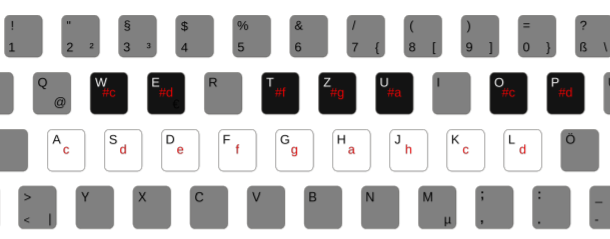
\includegraphics[width=70mm,scale=0.6]{keymap}
Die Tasten \textbf{1,2} verändern die Tondauer. Mit den Tasten \textbf{Y,X} verändert sich die Octave und mit den Tasten \textbf{C,V} das Volumen.
\subsection*{USART}
USART steht für Universal Synchronous and Asynchronous Receiver-Transmitter. Das ist eine serielle Schnittstelle welche vor allem für interne Mikrocontroller Kommunikation verwendet wird. Ein wichtiger Aspekt bei USART ist die Baudrate. Die Baudrate wird wie folgt berechnet.
\setlength{\belowdisplayskip}{0pt} \setlength{\belowdisplayshortskip}{0pt}
\setlength{\abovedisplayskip}{0pt} \setlength{\abovedisplayshortskip}{0pt}
\[BR = \frac{f_{pclk} }{8*(2- OVER8) * USARTDIV}\]
\subsection*{PWM}
PWM steht für Pulse Width Modulation. Um verschieden Noten über den Speaker abspielen zu können, müssen wir die Signale wie auf der Grafik abgebildet anpassen. Diese Wellen werden dann mit Hilfe von PWM äquivalent auf den Speaker gegeben.
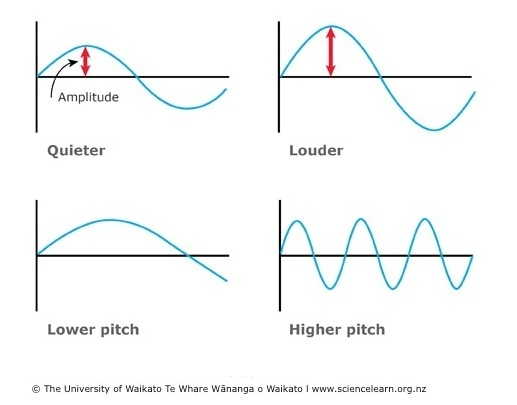
\includegraphics[width=40mm\\]{graphSound} 
\section*{Methology}
Zuerst muss der USART konfiguriert werden. Wichtig ist dabei die Baud Rate zu definieren. Mit der oben erwähnten Formel kann sie errechnet werden.
\begin{lstlisting}[style=CStyle]
//Set Baud Rate 115200 on a 16MHz ref clock
USART2->BRR = 0x45;
\end{lstlisting}
Um das gewünschte Verhalten zu implementieren wird bei jeder detektierten Eingabe vom USART ein Interrupt generiert. Dieses Interrupt startet das abspielen eines Tones bis eine gewisse Zeit abgelaufen ist. Diese Zeit wird vom Timer TIM7 gemessen. Er wird im One-Pulse Mode betrieben und generiert seiner seit nach einer definierten Zeit ein Interrupt. In dieser Interrupt Routine wird dann das abspielen des Tones wieder unterbrochen. 
\section*{Results}
Das Resultat des vorliegenden Projekts ist ein funktionierendes Piano. Um das Piano zu bedienen benötigt der Nutzer eine serielle Schnittstelle. Eine bekannte ist Hterm. Für diese Anwendungen empfiehlt sich aber eine wie PuTTy. Sie erlaubt es unter Terminal/localEcho Einstellungen zu treffen. So werden Tasteneingaben direkt an den $\mu$C übertragen. So kann bei genügendem Talent auch wirklich Klavier gespielt werden. Im nachfolgenden Bild sehen sie noch wie sie die serielle Schnittstelle konfigurieren müssen.
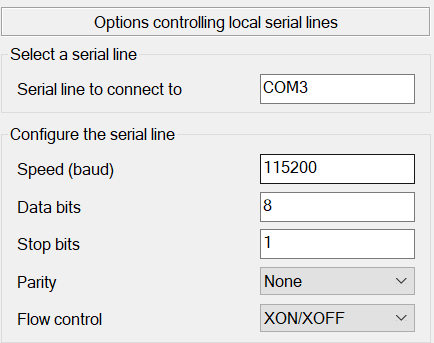
\includegraphics[width=70mm\\]{PuTTY} 
\newline Es gibt auch ein paar Punkte die besser sein könnten. Der Speaker limitiert die Range der angenehmen Töne. Sehr tiefe Töne fangen an zu Rattern und die Hohen Töne sind sehr unangenehm. \\
Wenn sie den Source Code meines Projektes ansehen möchten können sie das auf GitHub machen. \url{https://github.com/SebastianvonAllmen/Ex10.git}
\section*{Discussion}
\subsection*{Zum Projekt}
Ein Feature das ich noch implementieren möchte ist das abspielen eines gespeicherten Liedes. Es soll einen Knopf geben, mit welchem ein Lied abgespielt werden kann. So können auch musikalisch wenig talentierte Nutzer schöne Musik spielen. Ich möchte ein Python Skript schreiben welches mit einen String aus einem MIDI File generiert. Diesen String, kann ich dann als Song abspielen. 
\subsection*{Persönlich}
Für mich persönlich war das Projekt extrem lehrreich. Es war zu vielen Zeiten etwas frustrierend, weil ich z.B. vergessen habe eine Clock zu aktivieren, oder ein Interrupt einzuschalten. Diese Probleme zu debuggen ist zu beginn schwer. Ich merkte aber schnell wie ich besser darin wurde solche Probleme zu erkennen. Zudem ist es wichtig für mich eine saubere Arbeitsweise zu erlernen, wo solche Fehler nicht passieren. Dafür sind solche Aufgaben immer wichtig. Zudem war es das erste mal das ich einen Bericht in LaTeX schreibe. Auch diese Erfahrung ist für mich durchwegs positiv, auch wenn ich zu Beginn sehr skeptisch war. Durch die ausgearbeitete Vorlage fällt der Einstieg einfach. Die Foren online sind auch hilfreich.

\end{multicols}

  %------------ BIBLIOGRAPHY ---------------
%\printbibliography

\end{document}
